% !TEX root = ../ClassicThesis_DEIB.tex

\chapter{The GRAPE project} \label{chap:grapeProject}

In this chapter, we are going to give a description of the project this thesis work is part of, with particular emphasis on the parts that were specifically addresses in the thesis work. For the description of the project, we make reference to its official proposal.
\ac{GRAPE} is an experimental project of \ac{ECHORD++} and, as hinted in the first part of Chapter \ref{chap:backgroundAndToolsChapter}, it focuses on vineyard farming activities and aims at setting up a robotic manipulation platform able to support lead users to develop a variety of farming applications.
 In effect, the main goal of \ac{GRAPE} is not the complete development of an industrial platform, but, coherently with the research scenario:
\begin{enumerate}
	\item the development of example applications in the pre-mentioned context, exploiting and improving the so-called \textit{key enabling technologies} in robot navigation, perception and manipulation of the project partners; the resulting capabilities are likely to allow to make it easier for small and medium enterprises working in the fields of agricultural robots and, more in general, plant protection.
	\item increase of robot acceptance by farmers and agronomists: since the very last goal of this project is not about the pure research but about the enterprise world, particular attention is given into the realization of a robotic platform that could be accepted by potential end users. For this reason, a constant interaction between the project partners and the potential stakeholders (\textit{i.e.} vinegrowers) is mantained also in development phases.
\end{enumerate}

The example applications have been selected in order to challenge perception and action capabilities, to achieve vineyard monitoring, navigation and manipulation tasks. This decision is taken in the scope of turning traditional farming into precision farming; the realization of such a turn would allow for both the decrease of the chemical load in food and environment, and an improvements of profits and yield for farmers, that would get a return for this investment \parencite{precisionFarming}. The introduction of precision farming tecniques leads indeed to a lot of advantages, for example early detection of plants diseases, or application of pesticides and fungicides with high precision and only when needed.

It's clear that some of these high-precision tasks are still too complex to be automated, and current state-of-the-art in research and technology have been proved to be not yet mature to give rise to a commercial product able to compete with a skilled agricultural agent. The goal of \ac{GRAPE} is creating the enabling technologies to allow agricultural companies to develop vineyard robots to keep filling the gap that exists with respect to traditional methods.

\begin{figure}
	\centering
	\subfloat[]{%
		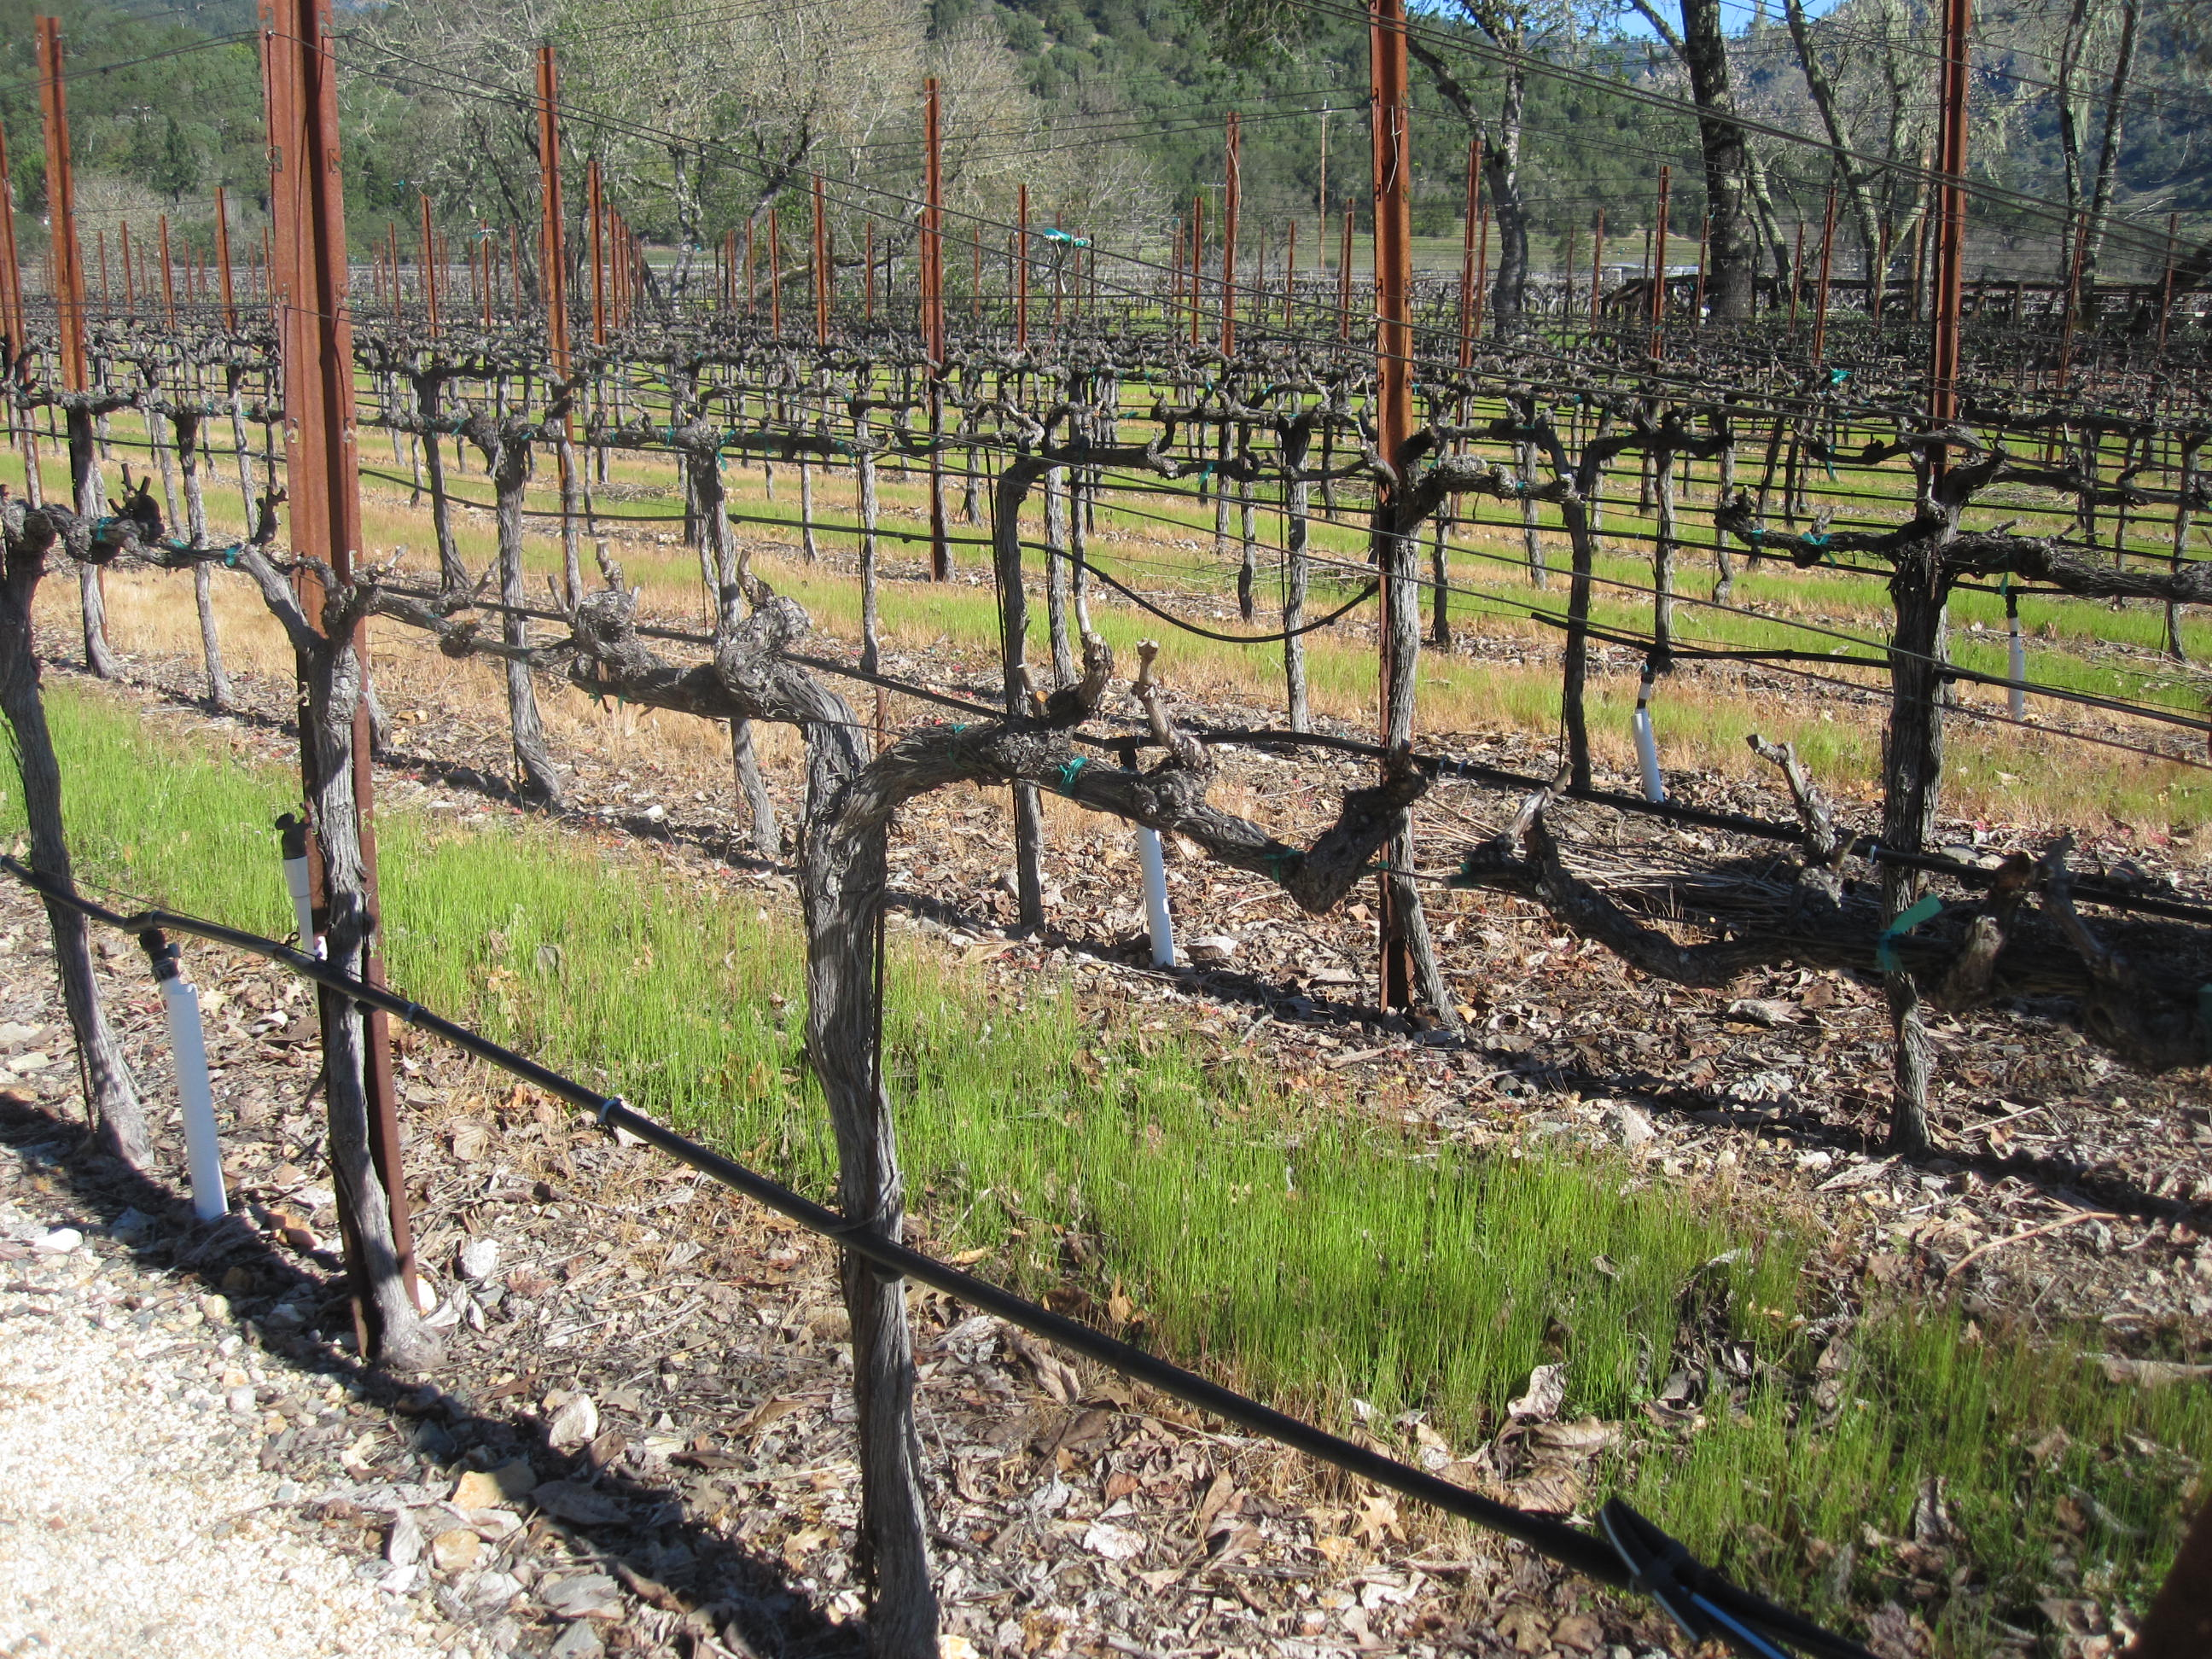
\includegraphics[width=0.35\textwidth]{Images/grape_project/prunedVine.jpg}
		\label{fig:vignaSenzaFoglie}}
	\qquad
	\subfloat[]{%
		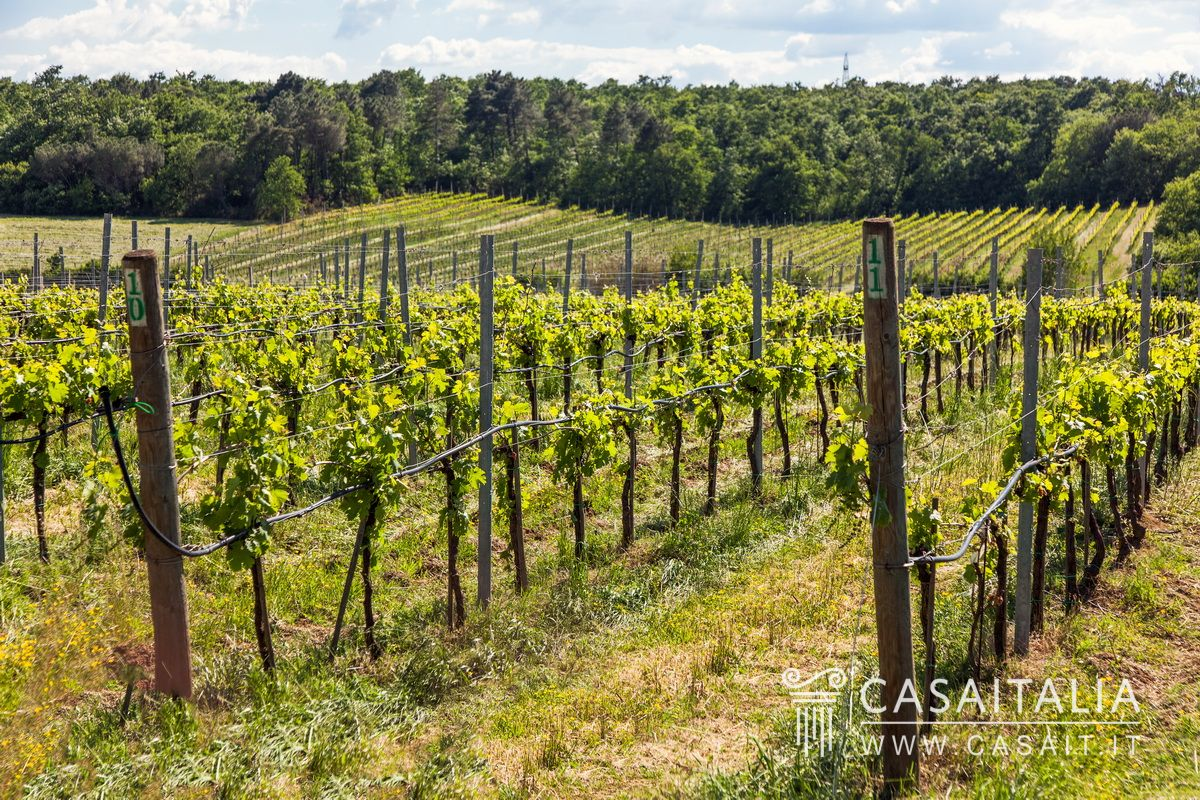
\includegraphics[width=0.36\textwidth]{Images/grape_project/leavesVine.jpg}
		\label{fig:vignaFoglia}}
	\caption{\textit{A vine before (\ref{fig:vignaSenzaFoglie}) and after (\ref{fig:vignaFoglia}) le} having leafed out.}
	\label{fig:vignaConSenzaFoglie}
\end{figure}


\ac{GRAPE} project specification identify these two application examples:
\begin{itemize}
	\item \textbf{Vineyard monitoring and autonomous navigation}: the developed robotic platform must be able to autonomously navigate the vineyard and localize itself into a map of the environment (downstream a mapping phase), to be able to monitor the state of the vineyard (\textit{e.g.} foliage and grapes inspection). The navigation The project implementation focused on a semi-autonomous monitoring, that consider a fully autonomous navigation platoform, with video stream capability that allows human users to observe in person the live data collected by the robot for assessment of crop condition. The localization and navigation parts, however, are a key point for any kind of tasks in the for an \ac{UGV} field robot, because of the probability of high slope ground, rugged terrain morphology and unstructured map. 
	\item \textbf{Autonomous application of pherormone dispenser applications}: pherormone dispensers are used for \textit{mating disruption} tecniques, to protect grapevines from grape moths, by disrupting the bugs' reproductive cycle making use of synthesized sex pherormones. Also in this case, the most relevant challenge is brought by the unstructured environment, that makes the sensing and manipulation tasks significantly harder.  However, note that pherormones deployment task gets easier if you think that the timing of the reproductive cycle (on which of course we have no control at all) forces this operation to be performed in a season where grape plants are pruned, and have not leafed out yet \parencite{mateDisruptionEfficiency}. Of course, the absence of foliage and grapes makes this task significantly easier (see Image \ref{fig:vignaConSenzaFoglie}).
\end{itemize}

For what concern the second goal of the project \textit{i.e.} a major commitment about the acceptance of the robotic system in a field that's still strongly led by traditional methods, its realization consists mostly in the creation of an user-friendly interface (possibly for smartphones or tablets) for the \ac{GRAPE} system, that allows an user to:
\begin{itemize}
	\item constantly and easily visualize the position and activity of the robot 
	\item perform supervisory control on the platform \textit{e.g.} selection of the plants for the dispensers deployment
	\item in case of a failure of the \ac{UGV} in an autonomous task, provide a teleoperation interface to carry out the operation
\end{itemize}
The whole project was also to be designed with and adequate degree of modularity, in order to naturally support the possible extension to a fleet of robot able to operate in parallel. Note that, as described in Section \ref{sec:robotOperatingSystem}, this goal gets very easy by the usage of \ac{ROS} framework.

The \ac{GRAPE} projects involved three partners, each with different assignments, and different responsibilities in the project context: \textbf{PoliMi}, \textbf{Eurecat} (a technology center located in Catalonia, that operates in many industrial and research fields, including robotics), and \textbf{Vitirover} (an agricultural robots company, located in France).
To make the different teams interact and test the compatibility of the develop parts, some communal sessions of integration and tests, that we'll call \textit{integration weeks}, have been carried out within the duration of the whole project. In this thesis we are going to focus mostly on the experiments and results carried out during the last \ac{GRAPE} integration week, held in Marc 2018.

\begin{figure}
	\centering
	\subfloat[]{%
		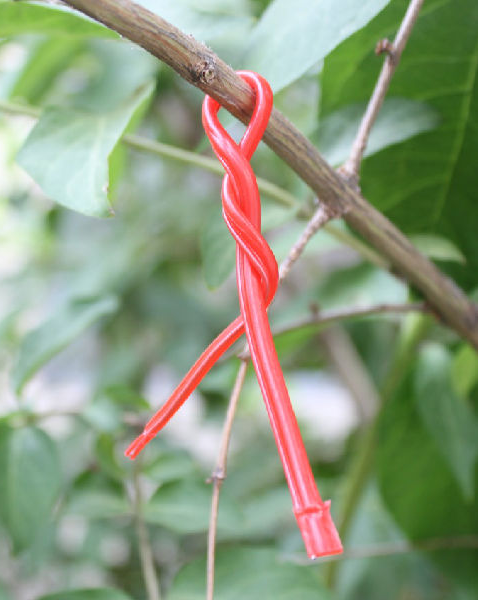
\includegraphics[width=0.3\textwidth]{Images/grape_project/dispenser1.png}
		\label{fig:dispenser1}}
	\qquad
	\subfloat[]{%
		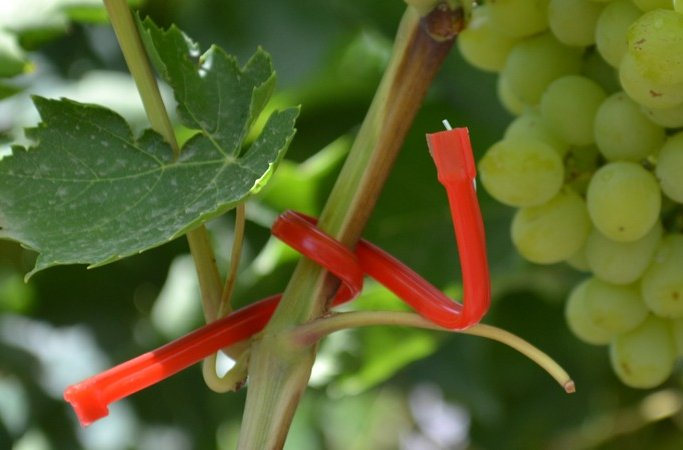
\includegraphics[width=0.3\textwidth]{Images/grape_project/dispenser2.jpg}
		\label{fig:dispenser2}}
	\qquad
	\subfloat[]{%
		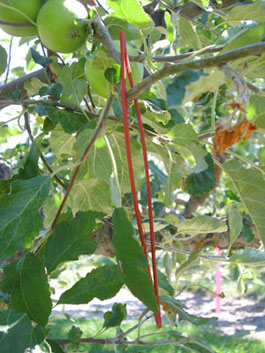
\includegraphics[width=0.12\textwidth]{Images/grape_project/dispenserNostro.jpg}
		\label{fig:dispenserNostro}}
	\caption{\textit{Different shape of pherormone dispensers available on the market. The model used in \ac{GRAPE} is the one depicted in image \ref{fig:dispenserNostro}}}
	\label{fig:dispensers}
\end{figure}

The problems tackled in this thesis are a subset of the ones assigned to PoliMi in the project proposal; for our work we took advantages from the preceding work and analysis described in \cite{grapeAltroPaper}. These aspects are:
\begin{itemize}
	\item design of the overall software architecture, in the \ac{ROS} framework
	\item revision and enhancement of the mapping, localization and navigation systems
	\item design and part of the implementation of the pherormone dispenser application
\end{itemize}

We are presenting a short list of EU projects related to robotics for precision farming, with direct or indirect application to vineyards. All these projects have been developed in the last 5 years, and demonstrate the growing interest of the scientic community and potential end users to this application and research field.

\begin{figure}
	\centering
	\subfloat[]{%
		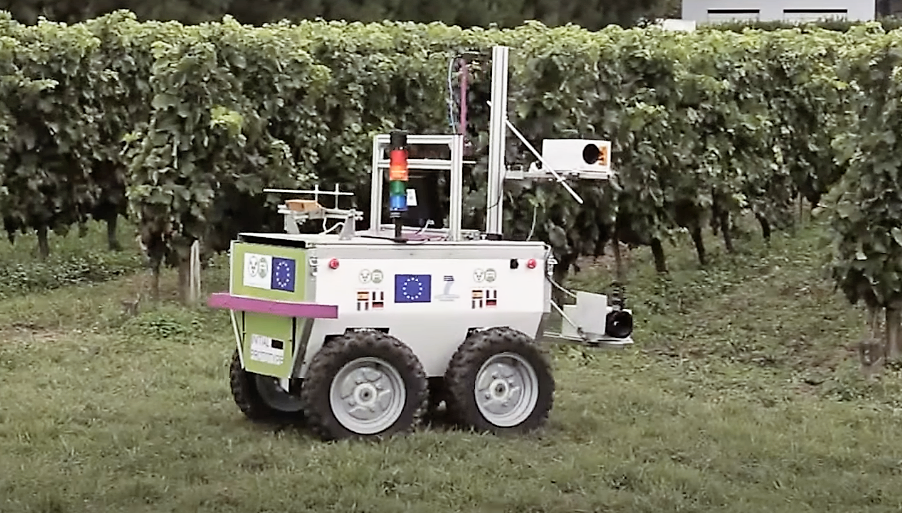
\includegraphics[width=0.55\textwidth]{Images/grape_project/vinerobot.png}
		\label{fig:vinerobot}}
	\qquad
	\subfloat[]{%
		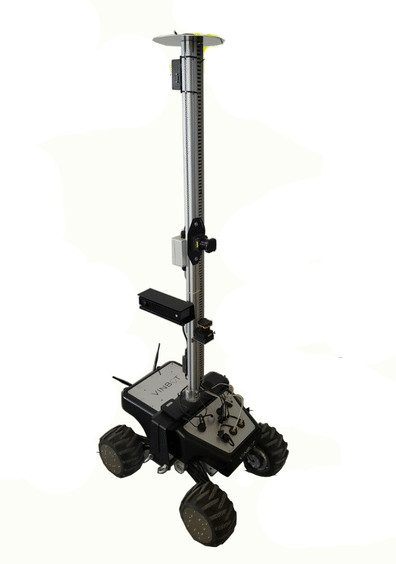
\includegraphics[width=0.3\textwidth]{Images/grape_project/vinbot.jpg}
		\label{fig:vinbot}}
	\caption{\textit{Other field robots developed in EU projects in the last 6 years: \ref{fig:vinerobot} Vinerobot, \ref{fig:vinbot} Vinbot.}}
\end{figure}

\begin{description}
	\item[VINEROBOT] Automated measurement and monitoring of parameters such as grape yield, vegetative growth, water status and grape composition in vineyards by use of an \ac{UGV} (see Figure \ref{fig:vinerobot}) endowed with artificial intelligence with sensing technologies. Chlorophyll-based fluorescence, RGB machine vision and thermography technologies are used to monitor vineyard on-the-go \parencite{vinerobot}.
	\item[VINBOT] Creation of an all-terrain autonomous mobile robot (see Figure \ref{fig:vinbot}) with a set of sensors capable of capturing and analysing vineyard images togethere with 3D data, by means of cloud computing applications, to determine the yield of vineyards and to share information with the winegrowers, in order to mix the grapes of homogeneous quality to efficiently market a range of wines by quality and price.
	\item[RHEA]
	\item[SWEPPER]
\end{description}

\begin{figure}
	\centering
	\subfloat[]{%
		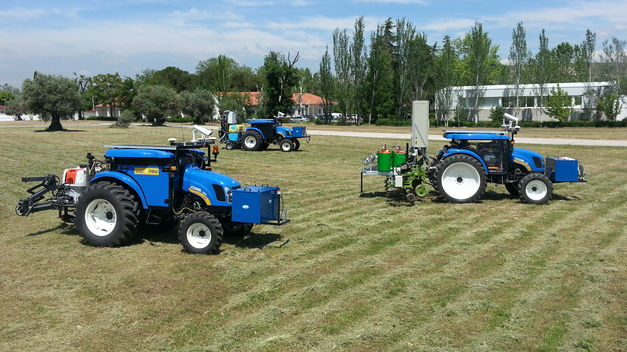
\includegraphics[width=0.5\textwidth]{Images/grape_project/rhea.jpg}
		\label{fig:rhea}}
	\qquad
	\subfloat[]{%
		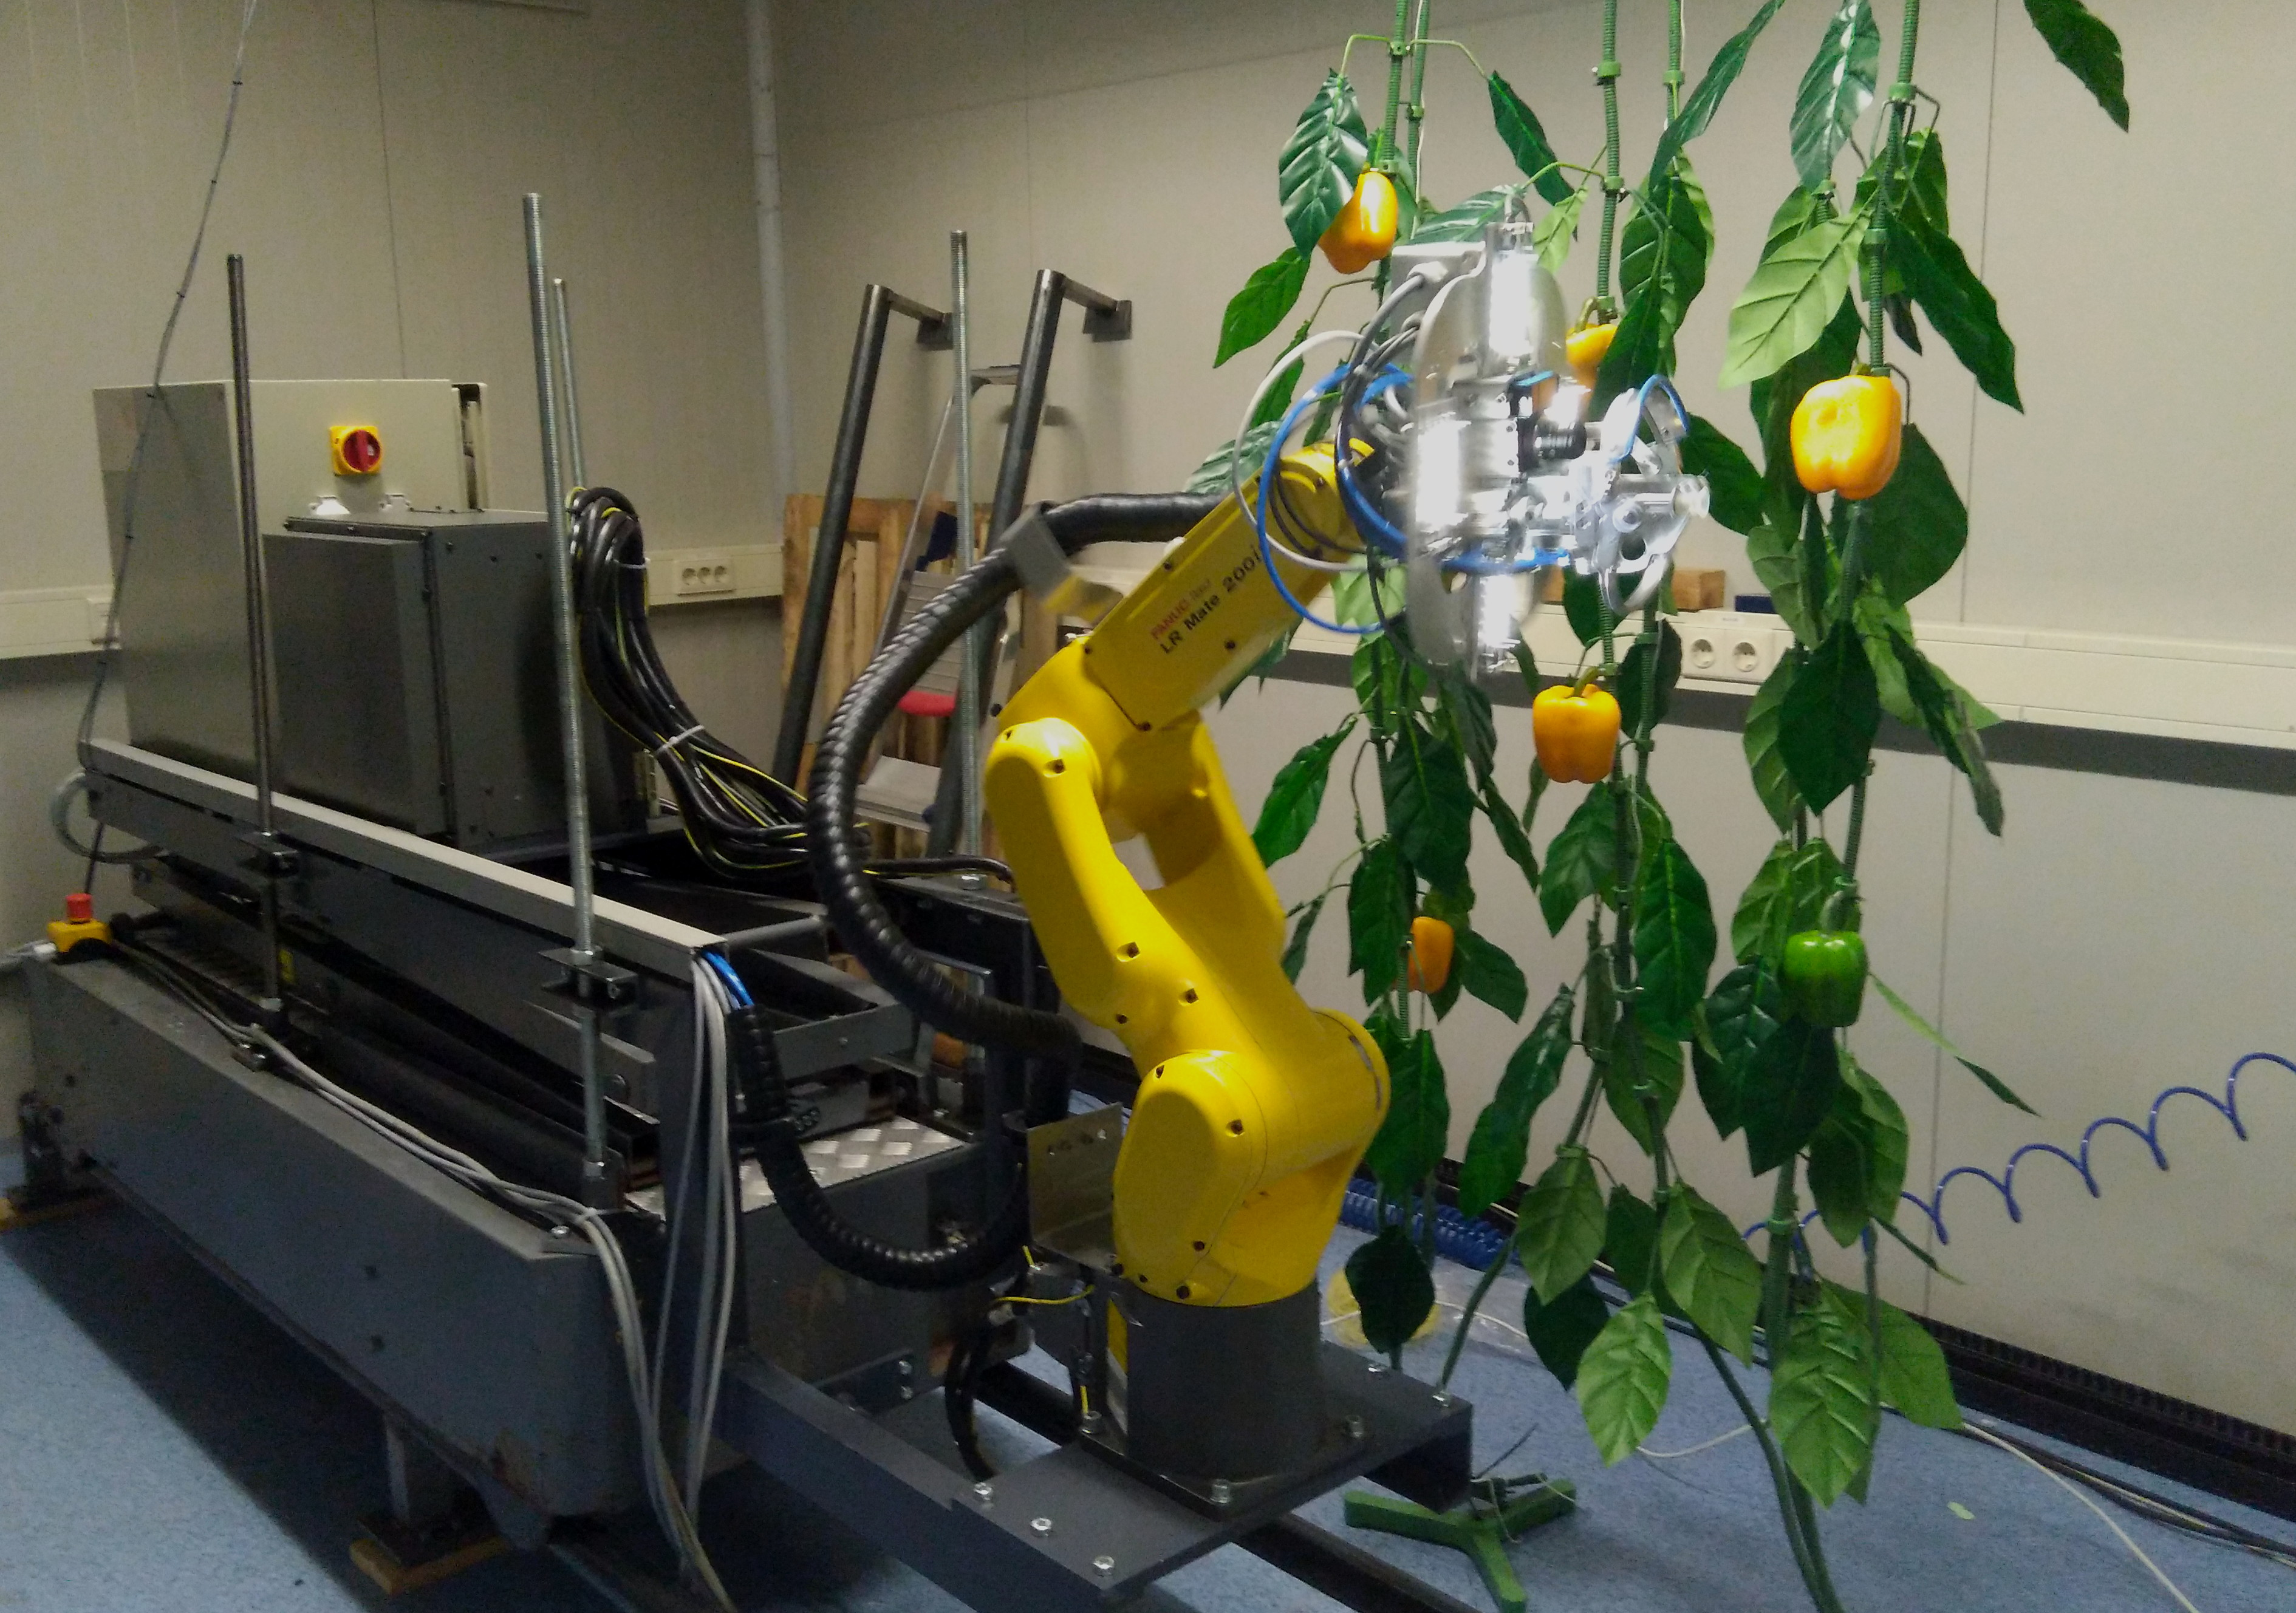
\includegraphics[width=0.4\textwidth]{Images/grape_project/swepper.jpg}
		\label{fig:swepper}}
	\caption{\textit{Other field robots developed in EU projects in the last 6 years: \ref{fig:vinerobot} Rhea, \ref{fig:vinbot} Swepper.}}
\end{figure}

